\newpage
\appendix
\crefalias{section}{appendix}
% supplementary material
In the appendix, we provide extra experimental results (\cref{app:extra_res}, including running time), ablations on a larger training set (\cref{app:extra_abla}), further analysis on $\mathcal{Q}_s$ (\cref{app:qs_analysis}), additional baseline (\cref{app:baseline}) and implementation (\cref{app:anchor}) details. We also provide visualization examples (\cref{app:example}).
\section{Extra Results} \label{app:extra_res}
In \cref{tab:ssv1},  we show the result of \method{} and baselines on ScreenSpot-v1~\citep{cheng2024seeclick}. In \cref{tab:time},  we compare the inference and training time between \method{}-3B and GUI-Actor-3B.

\section{Extra Ablations} \label{app:extra_abla}
In \cref{tab:results_with_verifier}, we compare the performance of \method{} and GUI-Actor, with both combined with the multi-region verifier proposed by GUI-Actor, showing that \method{} can benefit to the same extent as GUI-Actor from the extra verifier.  In~\cref{tab:ablation_all}, we add extra ablation results with variants trained on the 85k training set of \method{}-lite. It includes the results of uniform multi-head weighting with/without $\texttt{<ANCHOR>}$ token, vanilla attention grounding using multi-head weighting with $\mathcal{Q}'=\mathcal{Q}$ in \cref{eq:unified_head_score}, \method{}-3B-lite with stop-gradient on multi-head weights, GUI-Actor-3B with/without distance-aware labeling. The extra ablation results using a larger ablation training set are consistent with the results in \cref{tab:ablation}.

% \input{sec/app_multi_agent}
\section{Analysis for Visual-sink Query Token} \label{app:qs_analysis}
From ablation results in \cref{sec:ablation}, the global pattern indicated from the visual-sink query token computed $\mathcal{Q}_s$ from hidden states achieved better performance, supporting our selection that complies with the visual-query pattern from hidden states for weighting attention grounding.

In \cref{fig:visual_token}, we compute the similarity values between the multi-head weight vector computed from $\texttt{<ANCHOR>}$ token as the $\mathcal{Q}'=\{\texttt{<ANCHOR>}\}$ variant in \cref{eq:unified_head_score} and computed from each query token $q_i$ as $w_{l,h}=\sum_{v_i \in \mathcal{V}}\,\mathbf{A}^{l,h}_{q_i,v_i}$ from the trained \method{} model. The top-1 visual-sink query token consistently has the most similar multi-head weight vector with it computed from $\texttt{<ANCHOR>}$, supporting our design that computing $w_{l,h}$ from the visual-sink query token instead of $\texttt{<ANCHOR>}$ token, as it can work similarly with $\texttt{<ANCHOR>}$ in computing multi-head weight vector but avoiding the bias from random initialized $\texttt{<ANCHOR>}$ token.
\begin{table*}[!t]
    \centering
    \footnotesize
    \caption{Performance comparison of different models across various task categories based on Mobile, Desktop, Web and Average scores on \textbf{ScreenSpot-v1}.}
    % \vspace{-1em}
    \resizebox{0.9\linewidth}{!}{
    {
    \begin{tabular}{clccccccc}
        \toprule
        & \multirow{3}{*}{\textbf{Model}} 
          & \multicolumn{2}{c}{\textbf{Mobile}}
          & \multicolumn{2}{c}{\textbf{Desktop}}
          & \multicolumn{2}{c}{\textbf{Web}}
          & \multirow{2.5}{*}{\textbf{Avg.}} \\
        \cmidrule(lr){3-4}\cmidrule(lr){5-6}\cmidrule(lr){7-8}
        & & Text & Icon & Text & Icon & Text & Icon &  \\
        \midrule
        % \multirow{4}{*}{\rotatebox{90}{\bf General}}
        &GPT-4 & 22.6 & 24.5 & 20.2 & 11.8 & 9.2 & 8.8 & 16.2 \\
        &GPT-4o & 20.2 & 24.9 & 21.1 & 23.6 & 12.2 & 7.8 & 18.3 \\
        &Claude Computer Use & - & - & - & - & - & - & 83.0 \\
        &Gemini 2.0 & - & - & - & - & - & - & 84.0 \\
        % \midrule
        \midrule
        \multirow{6}{*}{\rotatebox{90}{\bf 3B}}
        &UGround-V1-2B & 89.4 & 72.0 & 88.7 & 65.7 & 81.3 & 68.9 & 77.7\\
        &UI-TARS-2B & 93.0 & 75.5 & 90.7 & 68.6 & 84.3 & 74.8 & 82.3 \\
        % \midrule
        &GUI-Actor-2B (Qwen2-VL) & 93.0 & 79.9 & 88.1 & 78.6 & 90.9 & 84.0 & 86.5 \\
        &GUI-Actor-3B (Qwen2.5-VL) & 94.5&83.8&92.8&82.1&91.3&82.5&88.4 \\
        \cmidrule(lr){2-9}
        &\textbf{\method{}-3B-lite} & 97.1&82.1&95.4&83.6&90.9&80.6&\textbf{88.8} \\
        \midrule
        \multirow{13}{*}{\rotatebox{90}{\bf 7B}}
        &Qwen2-VL-7B & 75.5 & 60.7 & 76.3 & 54.3 & 35.2 & 25.7 & 55.3 \\
        &CogAgent-7B & 67.0 & 24.0 & 74.2 & 20.0 & 70.4 & 28.6 & 47.4 \\
        &SeeClick-9.6B & 78.0 & 52.0 & 72.2 & 30.0 & 55.7 & 32.5 & 53.4 \\
        &Magma-8B & 60.4 & 58.5 & 75.3 & 52.9 & 69.1 & 52.0 & 60.3\\
        &Aguvis-G-7B & 88.3 & 78.2 & 88.1 & 70.7 & 85.7 & 74.8 & 81.8 \\
        &OS-Atlas-7B & 93.0 & 72.9 & 91.8 & 62.9 & 90.9 & 74.3 & 82.5 \\
        &Aguvis-7B & 95.6 & 77.7 & 93.8 & 67.1 & 88.3 & 75.2 & 84.4 \\
        &UGround-v1-7B & 93.0 & 79.9 & 93.8 & 76.4 & 90.9 & 84.0 & 86.3 \\
        &SparkUI-Parser&94.9&83.8&95.9&80.7&89.6&82.9&88.0\\
        &UI-TARS-7B & 94.5 & 85.2 & 95.9 & 85.7 & 90.0 & 83.5 & 89.5 \\
        &GUI-Actor-7B (Qwen2-VL)& 94.9 & 82.1 & 91.8 & 80.0& 91.3 & 85.4 & 88.3 \\
        &GUI-Actor-7B (Qwen2.5-VL) & 96.3&85.2&95.4&82.9&90.4&85.4&\textbf{89.9} \\
        \midrule
        \multirow{3}{*}{\rotatebox{90}{\bf 72B}}
        &UI-TARS-72B & 94.9 & 82.5 & 89.7 & 88.6 & 88.7 & 85.0 & 88.4 \\
        &Aguvis-72B & 94.5 & 85.2 & 95.4 & 77.9 & 91.3 & 85.9 & 89.2 \\
        &UGround-V1-72B & 94.1 & 83.4 & 94.9 & 85.7 & 90.4 & 87.9 & \textbf{89.4}\\
        \bottomrule
    \end{tabular}
    }
    }
    % \vspace{-2em}
    \label{tab:ssv1}
\end{table*}
\begin{table*}[!t]
    \centering
    \footnotesize
    \caption{Inference and training time (85k training set) comparison between \method{}-3B and GUI-Actor-3B.}
    \vspace{-1em}
    % {\color{blue}
    \begin{tabular}{lcc}
    \toprule
    & \textbf{GUI-Actor-3B} & \textbf{\method{}-3B} \\ 
    \midrule
    ScreenSpot-v2 (s/iteration)  &0.73  & 0.76 \\
    ScreenSpot-Pro (s/iteration) &1.72  & 1.76 \\
    OSWorld-G (s/iteration)      &1.15  &1.23  \\
    \midrule
    Training time (A100 GPU-hours) & $\sim260$ & $\sim192$\\
    \bottomrule
\end{tabular}
    
    % \vspace{-2em}
    \label{tab:time}
\end{table*}
\begin{table*}[!t]
    \centering
    \footnotesize
    \caption{Ablation results of \method{}-lite and GUI-Actor~\citep{wu2025gui} using the grounding verifier of GUI-Actor on ScreenSpot-v1 and ScreenSpot-v2.}
    \vspace{-1em}
    \resizebox{0.9\linewidth}{!}{
    % {\color{blue}
    \begin{tabular}{clccccccc}
        \toprule
        & \multirow{3}{*}{\textbf{Model}} 
          & \multicolumn{2}{c}{\textbf{Mobile}}
          & \multicolumn{2}{c}{\textbf{Desktop}}
          & \multicolumn{2}{c}{\textbf{Web}}
          & \multirow{2.5}{*}{\textbf{Avg.}} \\
        \cmidrule(lr){3-4}\cmidrule(lr){5-6}\cmidrule(lr){7-8}
        & & Text & Icon & Text & Icon & Text & Icon &  \\
        \midrule
        &GUI-Actor-3B (Qwen2.5-VL) + Verifier & 95.6&84.7&93.8&83.6&93.0&83.0&89.5$_{(+1.1)}$ \\
        &GUI-Actor-7B (Qwen2.5-VL) + Verifier & 96.0&85.6&96.4&82.9&91.7&83.0&\textbf{89.9}$_{(+0.0)}$\\
        &\textbf{\method{}-3B-lite} + Verifier & 97.1&83.8&96.4&83.6&91.3&84.0&\textbf{89.9}$_{(+1.1)}$ \\
        \midrule
        &GUI-Actor-3B (Qwen2.5-VL) + Verifier & 98.3 & 85.3 & 96.9 & 87.9 & 95.3 & 86.7 & 92.4$_{(+1.4)}$ \\
        &GUI-Actor-7B (Qwen2.5-VL) + Verifier & 96.9 & 89.6 & 97.4 & 86.4 & 95.7 & 84.7 & 92.5$_{(+0.4)}$ \\
        &\textbf{\method{}-3B-lite} + Verifier & 99.0&87.2&99.0&89.3&96.6&83.3&\textbf{93.0}$_{(+1.5)}$ \\
        \bottomrule
    \end{tabular}
    }
    % \vspace{-2em}
    \label{tab:results_with_verifier}
\end{table*}
\begin{table*}[!t]
    \centering
    \footnotesize
    \caption{Ablation results on ScreenSpot-v2, ScreenSpot-Pro and OSWorld-G of GUI grounding methods fine-tuned with the entire training set (254k elements). All variants are trained with the weighted patch-wise label introduced in \cref{sec:label} except $^*$.}
    \vspace{-1em}
    \resizebox{1\linewidth}{!}{
    % \begin{tabular}{y{240}ccccccc}
    \begin{tabular}{p{300pt}ccccccc}
        \toprule
        \multirow{2}{*}{\textbf{Model}} & \multicolumn{3}{c@{\hspace{1em}}}{\textbf{ScreenSpot-v2}} & \multicolumn{3}{c@{\hspace{1em}}}{\textbf{ScreenSpot-Pro}} & \multicolumn{1}{c@{\hspace{1em}}}{\textbf{OSWorld-G}}\\
        & Text & Icon & \textbf{Avg.}& Text & Icon & \textbf{Avg.} & \textbf{Avg.} \\
        \midrule
        GUI-Actor-3B$^*$ w/o weighted patch-wise label &94.99&80.87&88.84 & 49.13&19.04&37.63&50.53 \\
        GUI-Actor-3B &95.13&83.94&90.25&54.04&24.50&42.76&55.14\\
        \midrule
        \rowcolor{gray!10}\multicolumn{8}{l}{\textit{Attention Grounding without $\texttt{<ANCHOR>}$}}\\
        Vanilla Attention Grounding (multi-head weighting uniformly) &95.40&81.41&89.31& 58.03&21.52&44.09&55.03\\
        Vanilla Attention Grounding (multi-head weighted with $\mathcal{Q}'=\mathcal{Q}$ in \cref{eq:unified_head_score}) & 95.40&81.23&89.23 &55.07&23.84&43.14&54.14 \\
        \midrule
        \rowcolor{gray!10}\multicolumn{8}{l}{\textit{Simplified Attention Grounding with $\texttt{<ANCHOR>}$}}\\
        % \midrule
        $\texttt{<ANCHOR>}$-based multi-head weighting with $\mathcal{Q}'=\{\texttt{<ANCHOR>}\}$ in \cref{eq:unified_head_score}&96.52&82.85&90.57&59.77&21.69&45.22&54.79\\
        GUI-AIMA-3B-lite w/ stop-grad on $w$&96.38&85.56&\textbf{91.67}&58.34&25.33&45.73&56.38 \\
        GUI-AIMA-3B-lite &97.21&84.12&91.51& 62.03&29.97&\textbf{49.78}&\textbf{58.33} \\
        \bottomrule
      \end{tabular}}
    % \vspace{-2em}
    \label{tab:ablation_all}
\end{table*}
\begin{figure}
    \centering
    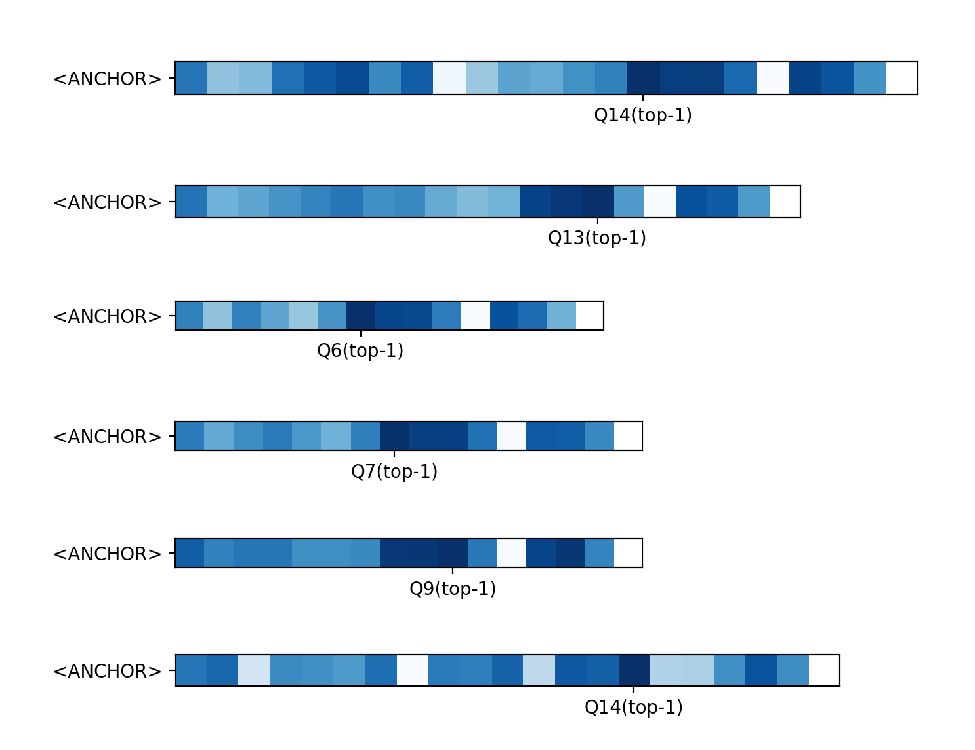
\includegraphics[width=0.8\linewidth]{sec/tab/visual_token.pdf}
    \caption{Cosine-similarity between multi-head attention vector computed between $\texttt{<ANCHOR>}$ and each text token. The top-1 visual-query token selected by \cref{eq:find_sink} consistently has the largest value with the $\texttt{<ANCHOR>}$ token.}
    \label{fig:visual_token}
\end{figure}
\section{Extra Details of ANCHOR Token Implementations} \label{app:anchor}
In \cref{sec:pre}, we abbreviate the implementation of $[\mathcal{V},\mathcal{Q},\texttt{<ANCHOR\_START>},\texttt{<ANCHOR>},\\\texttt{<ANCHOR\_END>}]$ as $[\mathcal{V},\mathcal{Q},\texttt{<ANCHOR>}]$ for brevity. For the single-area prediction setting in GUI grounding, we explore expanding a single $\texttt{<ANCHOR>}$ to multiple $\texttt{<ANCHOR>}$ tokens as $[\mathcal{V},\mathcal{Q},\texttt{<ANCHOR\_0>}, \texttt{<ANCHOR\_1>},\ldots,\texttt{<ANCHOR\_N>}]$ (abbreviate start and end tokens). However, it turns out to bring no performance gains and merely adds redundancy for the single-region grounding tasks. We will explore the multi-region grounding tasks with a disentangled $\texttt{<ANCHOR\_n>}$ token for each grounding region as future work.
\section{Baselines Details}\label{app:baseline}
Most baselines' results are taken from the original papers, except for GUI-G$^2$-3B, which is not reported in the source. Evaluation results of baselines for UI-Vision and MMBenchGUI-L2 in \cref{tab:ui_mm} are taken from the results reported in papers of UI-Venus-1.5~\citep{gao2026ui} and GroundNext~\citep{feizi2025grounding}.
\section{GUI Grounding Examples of \method{}}
\label{app:example}
We provide the visualizations of \method{}'s multi-head attention grounding results on ScreenSpot-v2 and ScreenSpot-Pro as follows in \cref{fig:example_v2}, \cref{fig:example_pro1,fig:example_pro2}.
\begin{figure}[t]
  \centering
  % 若想让小标题居中，可加：\captionsetup[subfigure]{justification=centering}
  \begin{subfigure}[t]{0.37\linewidth}
    \centering
    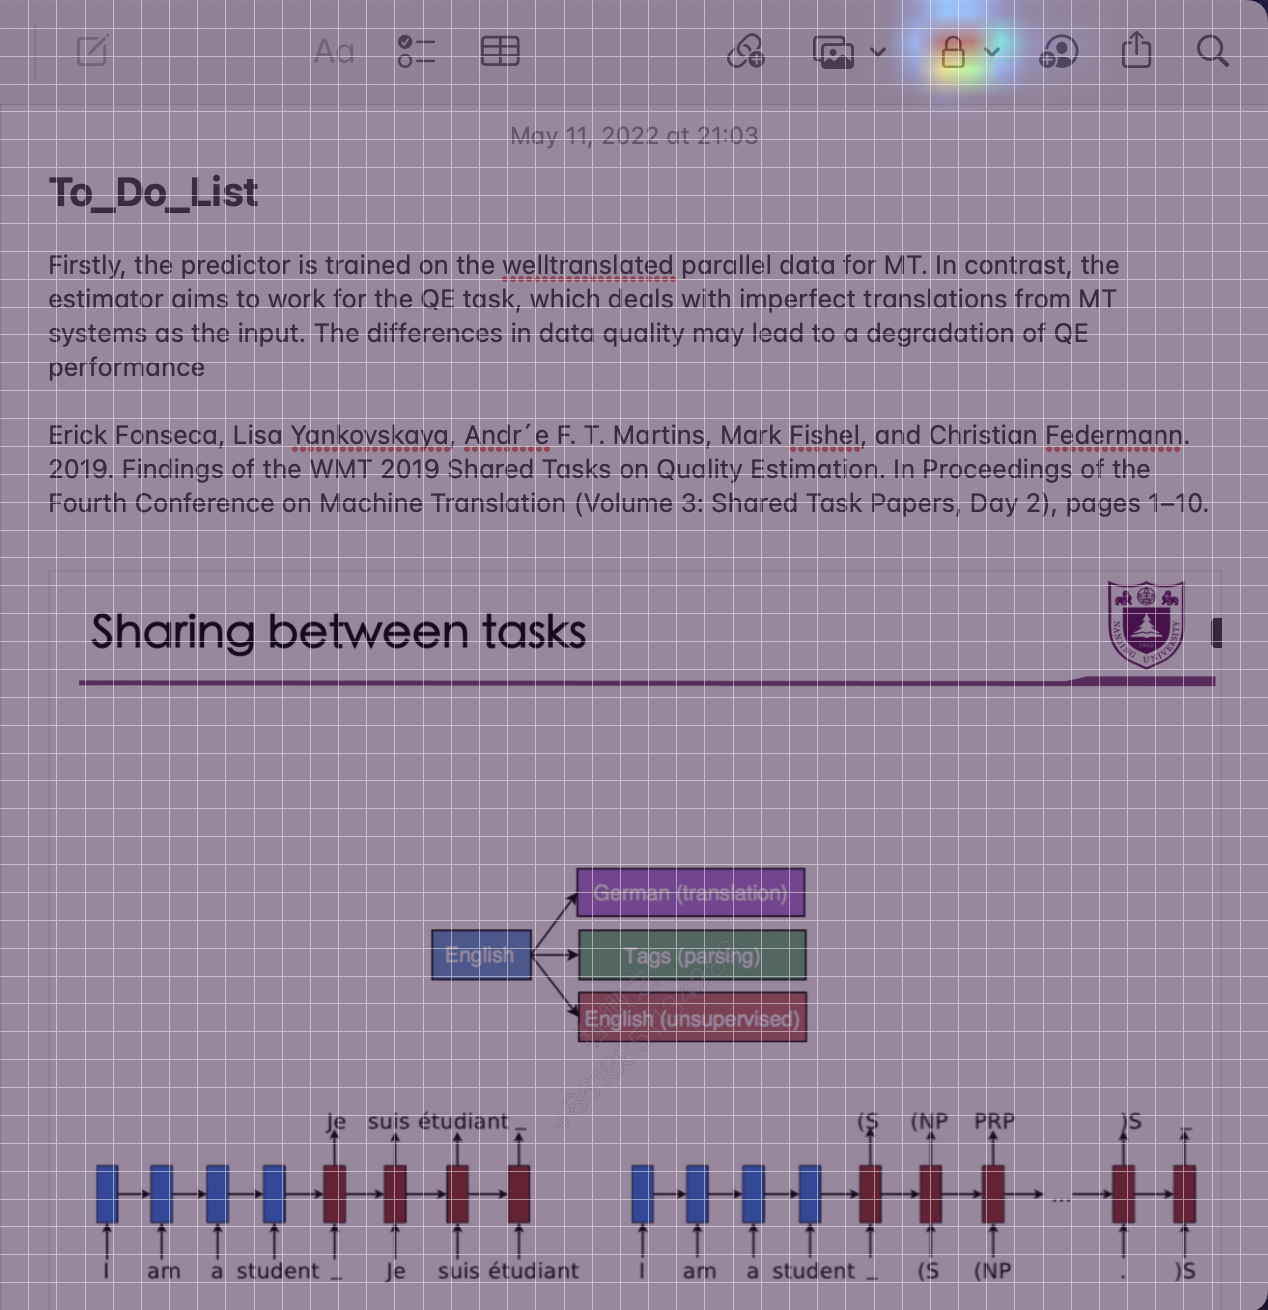
\includegraphics[width=\linewidth]{fig/vis_v2/lock.png} % 或 .png/.jpg
    \caption{Lock the memo.}
    \label{fig:v2_1}
  \end{subfigure}\hfill
  \begin{subfigure}[t]{0.37\linewidth}
    \centering
    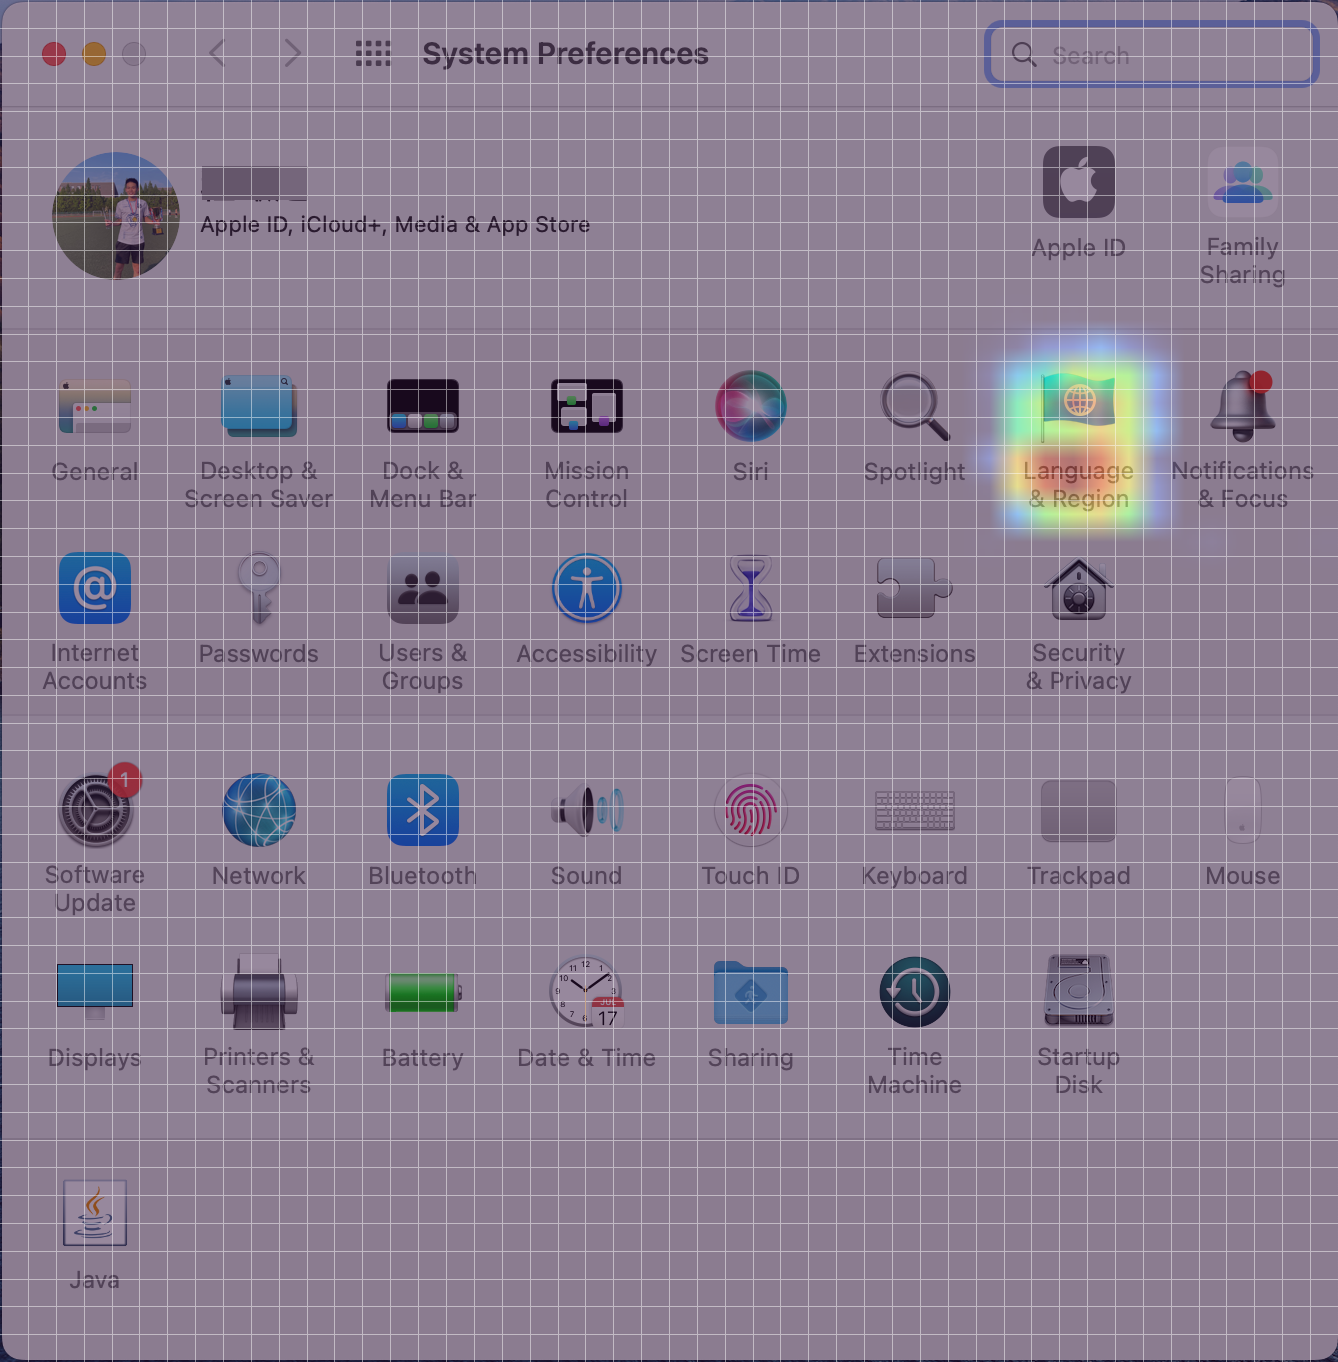
\includegraphics[width=\linewidth]{fig/vis_v2/view.png}
    \caption{View the language \& region settings.}
    \label{fig:v2_2}
  \end{subfigure}\hfill
  \begin{subfigure}[t]{0.25\linewidth}
    \centering
    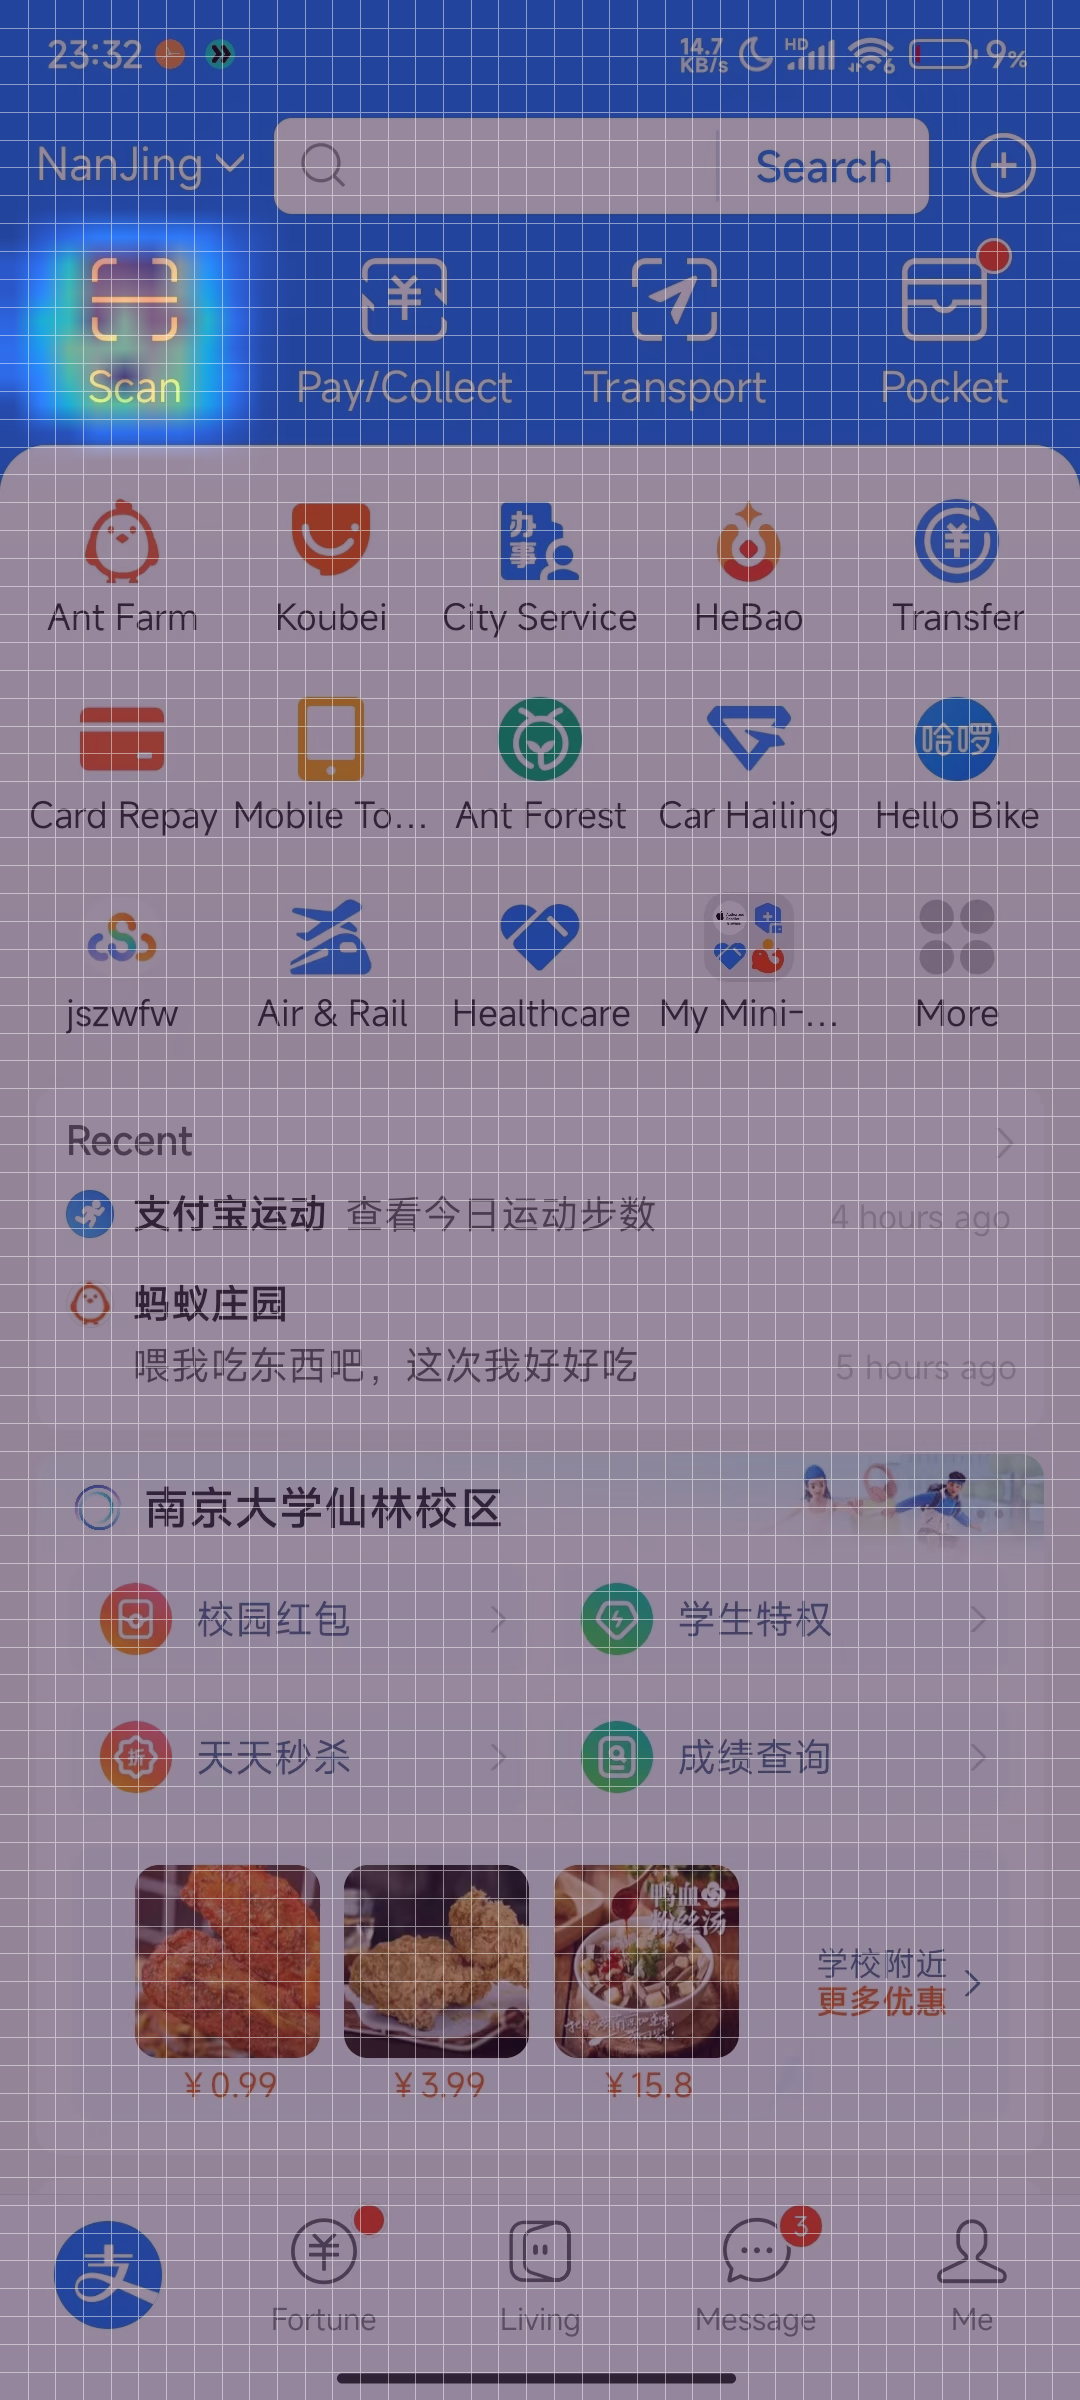
\includegraphics[width=\linewidth]{fig/vis_v2/scan.png}
    \caption{Scan QR code.}
    \label{fig:v2_3}
  \end{subfigure}
  % \vspace{0.6em} % 行间距，可按需调整
  % ----------- 第2行 -----------
  \begin{subfigure}[t]{0.54\linewidth}
    \centering
    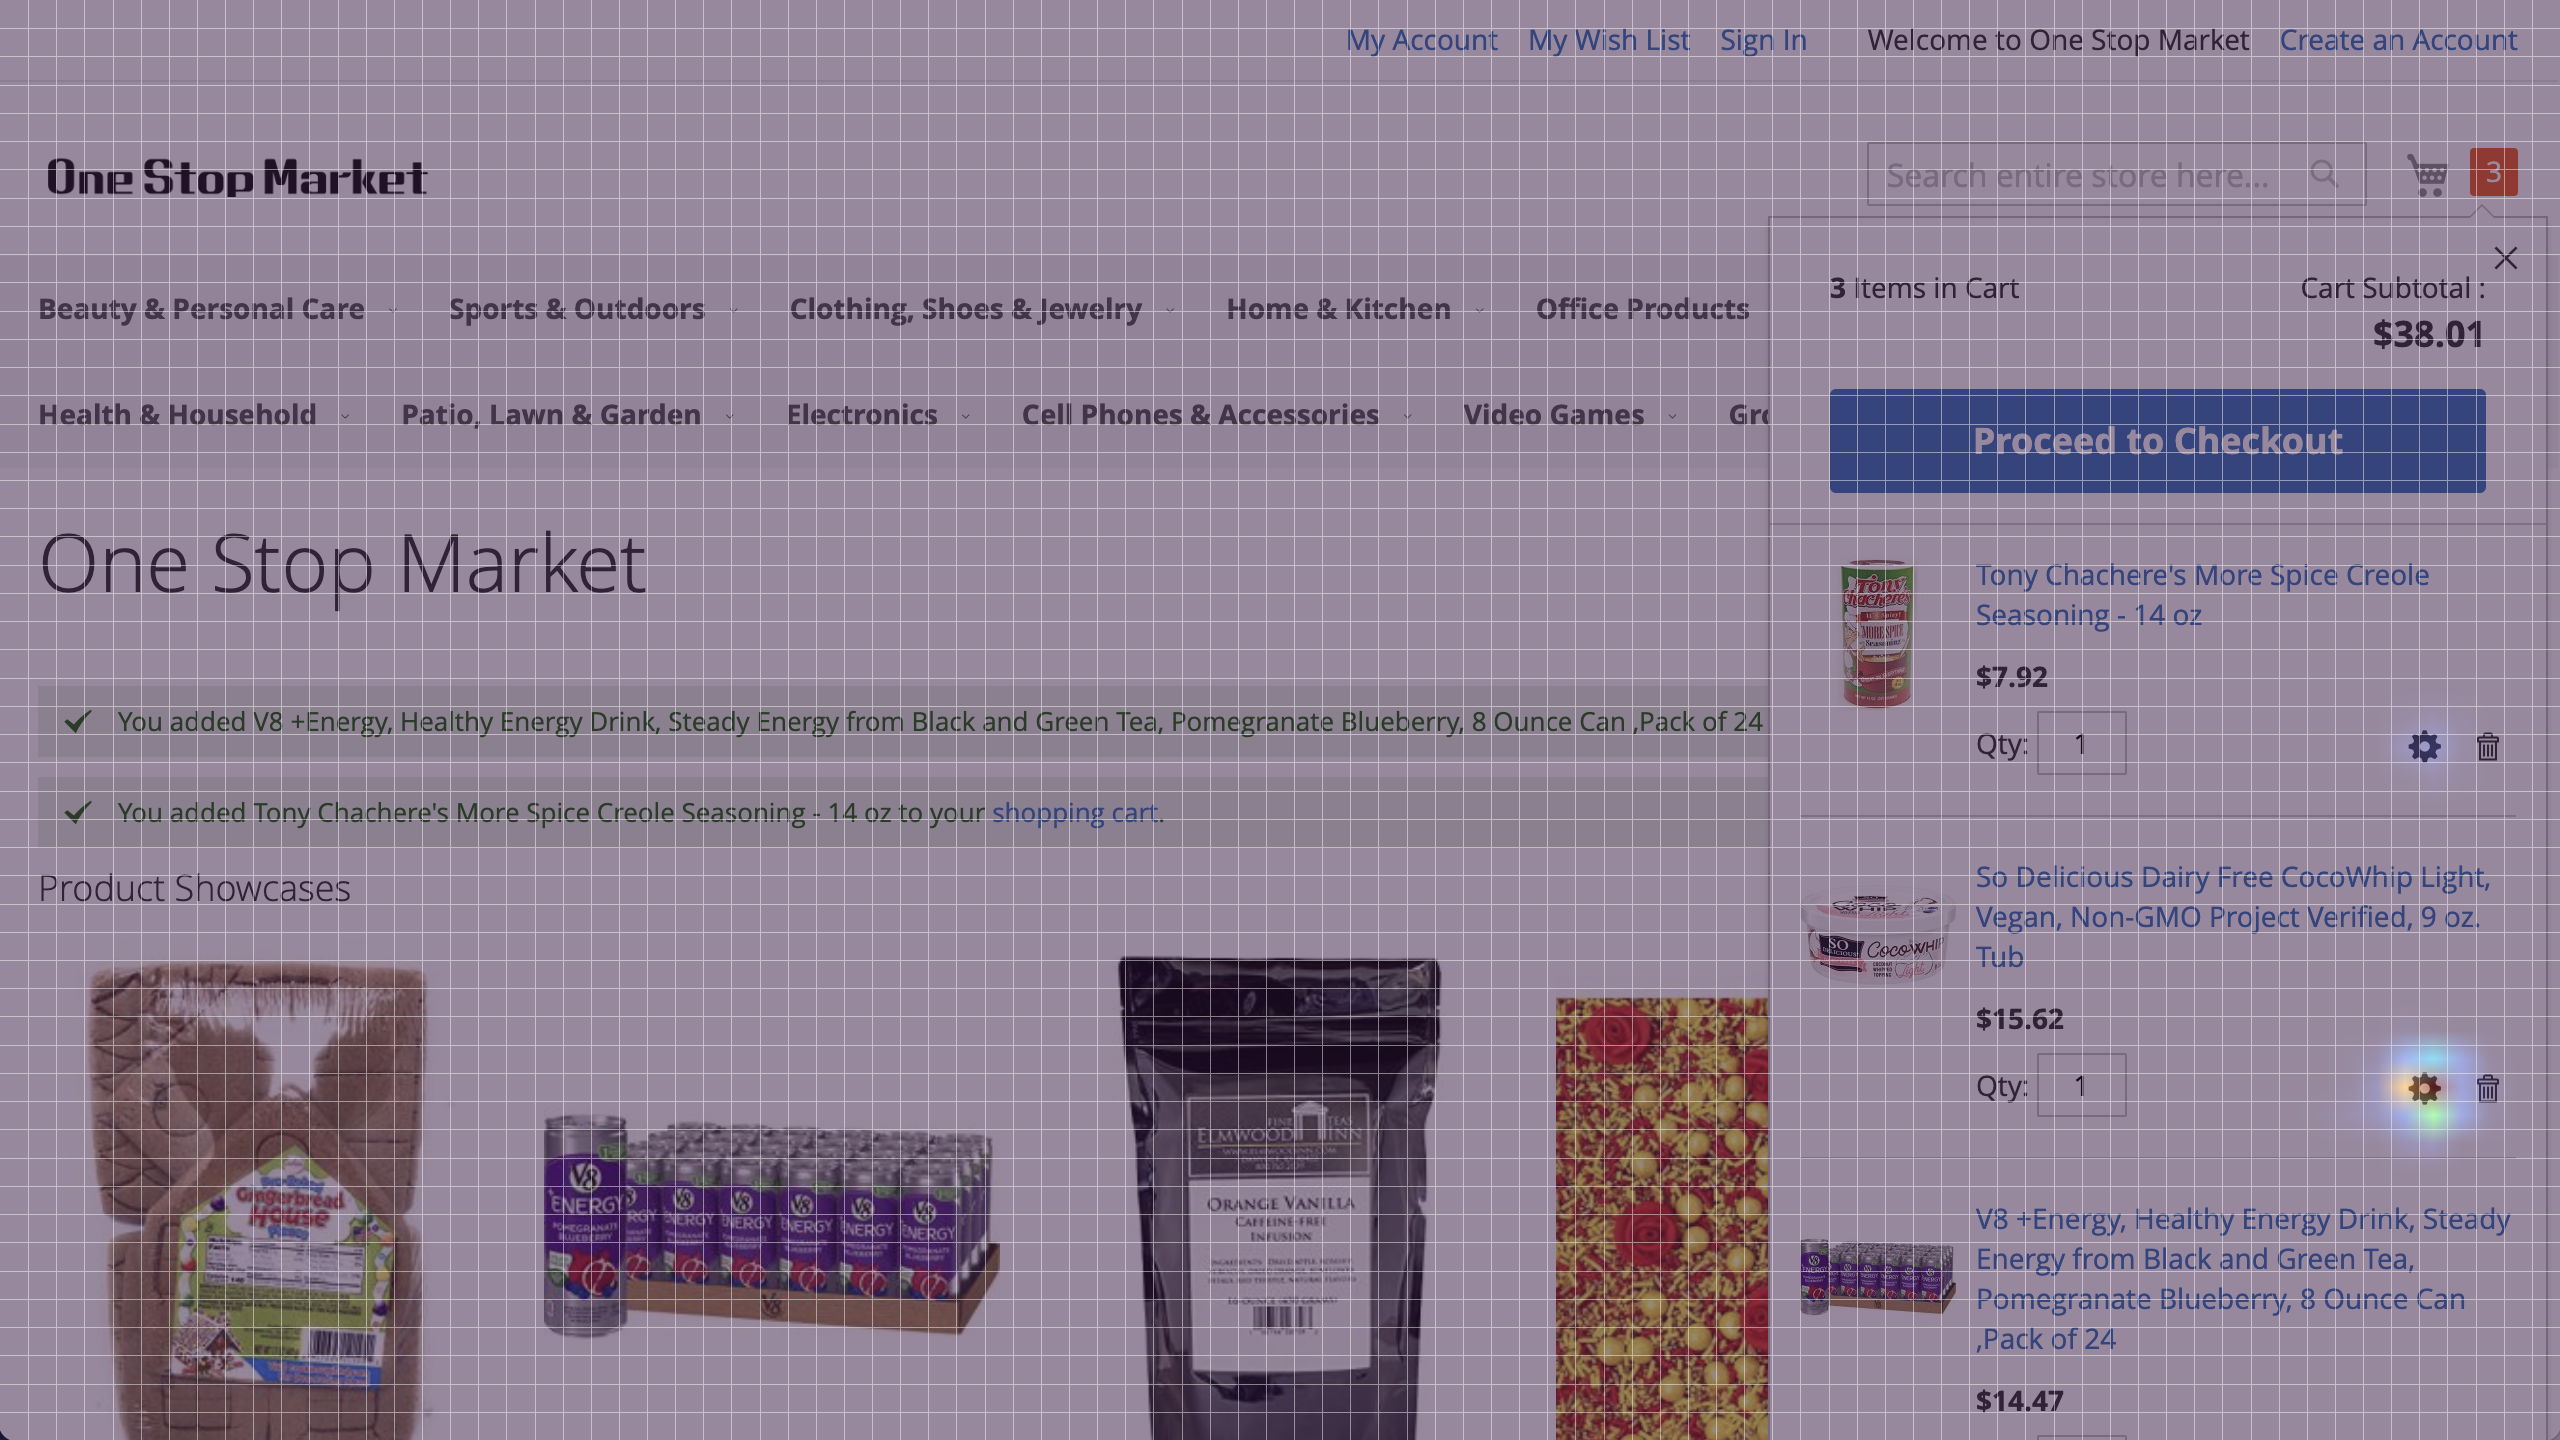
\includegraphics[width=\linewidth]{fig/vis_v2/settings.png}
    \caption{View settings of cocowhip light.}
    \label{fig:v2_4}
  \end{subfigure}\hfill
  \begin{subfigure}[t]{0.44\linewidth}
    \centering
    
\includegraphics[width=\linewidth]{fig/vis_v2/add.png}
    \caption{Add a new page.}
    \label{fig:v2_5}
  \end{subfigure}
  \caption{Visualization examples of \method{}'s grounding results on ScreenSpot-v2.}
  \label{fig:example_v2}
\end{figure}

\begin{figure}[!htbp]
\centering
\begin{subfigure}[b]{0.9\linewidth}
    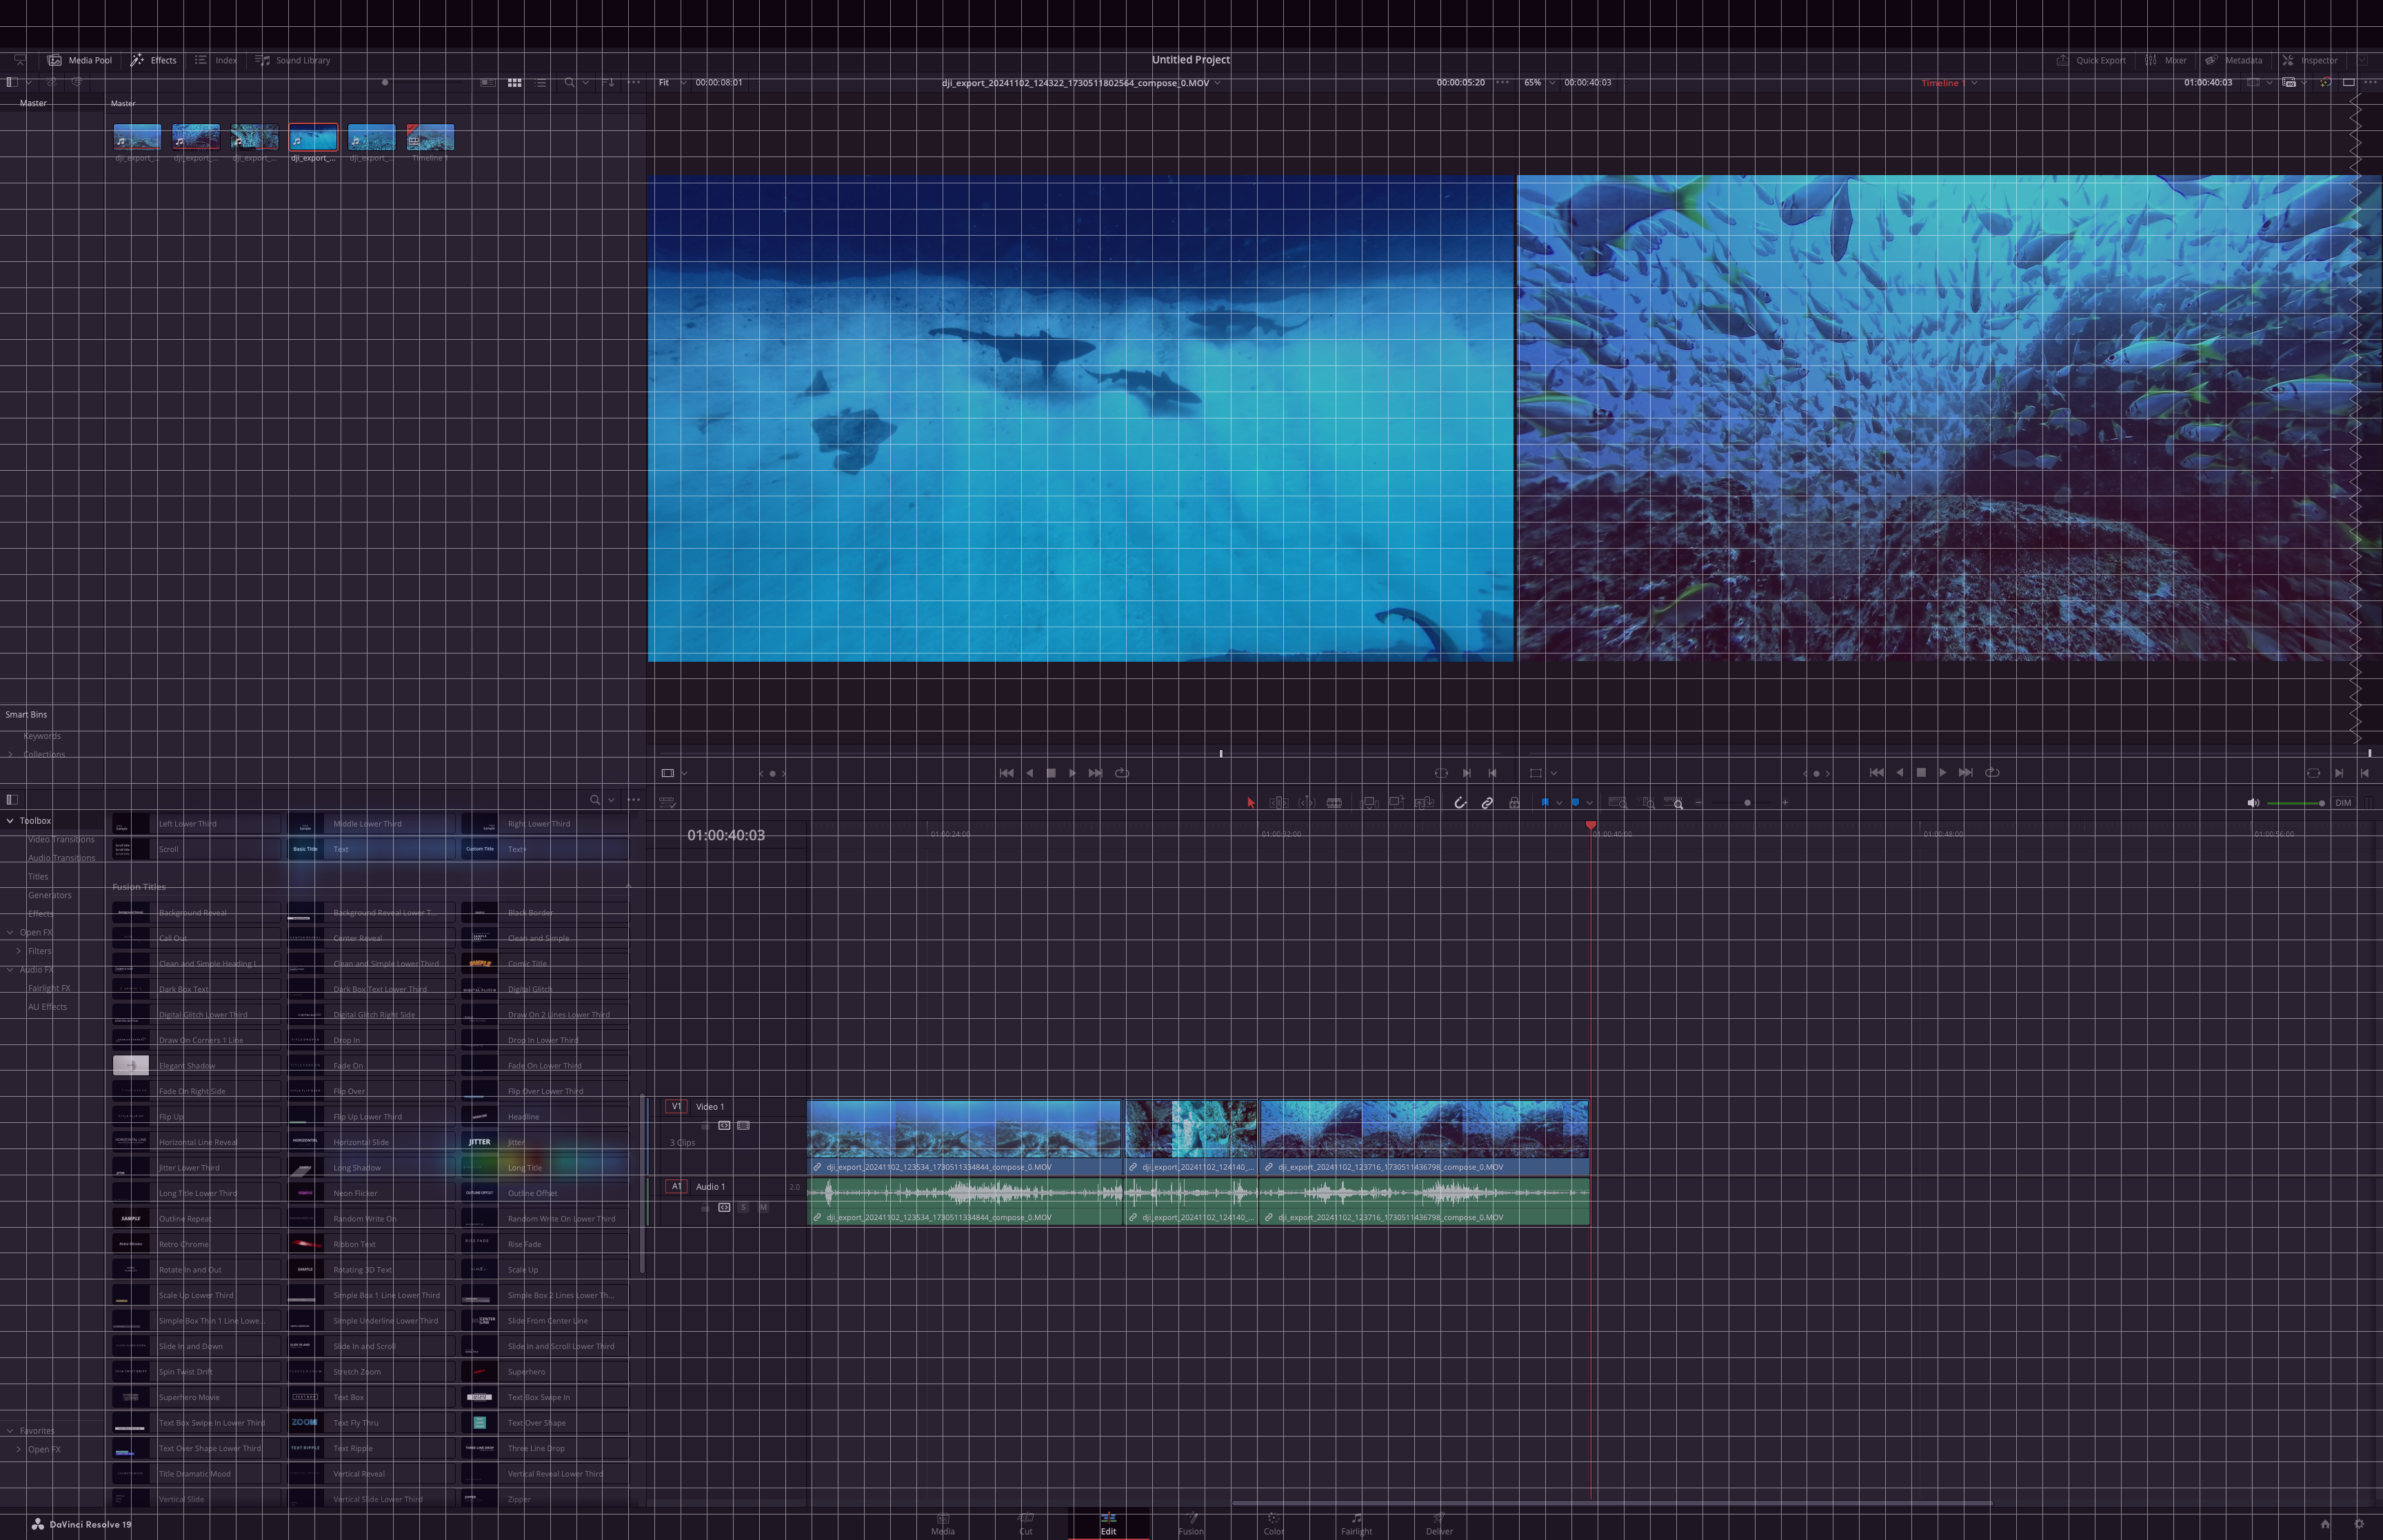
\includegraphics[width=\linewidth]{fig/vis_pro/add.png}
    \caption{Add long title.}
\end{subfigure}

\vspace{2pt}

\begin{subfigure}[b]{0.9\linewidth}
    \includegraphics[width=\linewidth]{fig/vis_pro/change.png}
    \caption{Change color theme in PyCharm.}
\end{subfigure}
\caption{Visualization examples of \method{}'s grounding results on ScreenSpot-Pro.}
\label{fig:example_pro1}
\end{figure}

\begin{figure}[!htbp]
\centering
\begin{subfigure}[b]{0.9\linewidth}
    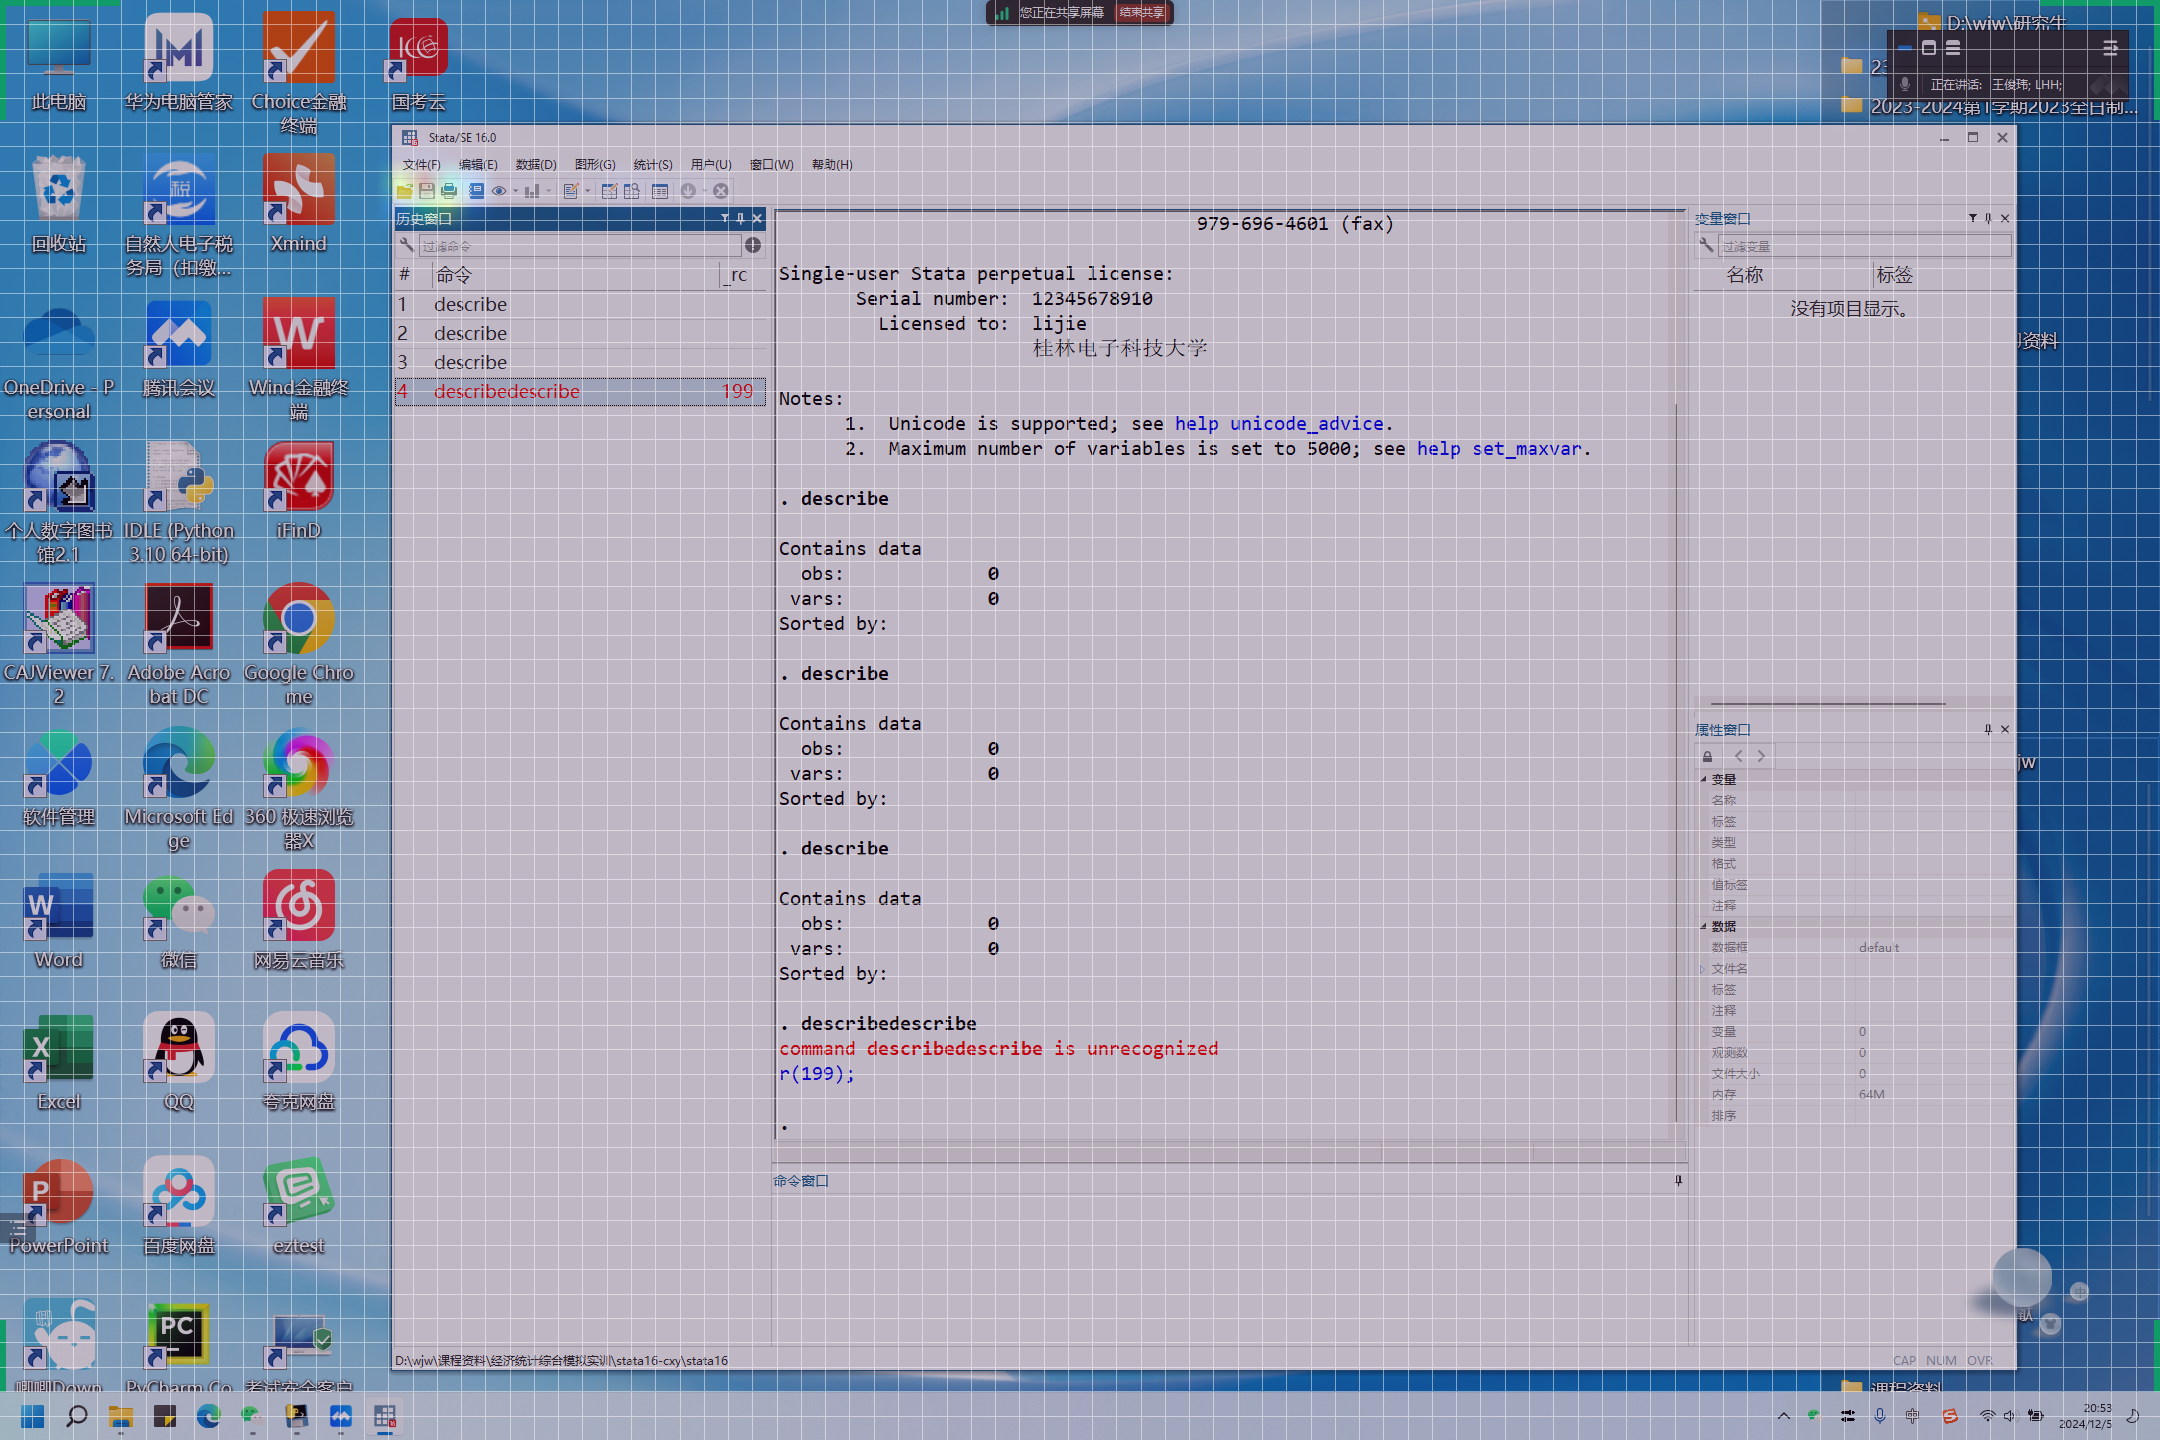
\includegraphics[width=\linewidth]{fig/vis_pro/save.png}
    \caption{Save a file.}
\end{subfigure}

\vspace{2pt}

\begin{subfigure}[b]{0.9\linewidth}
    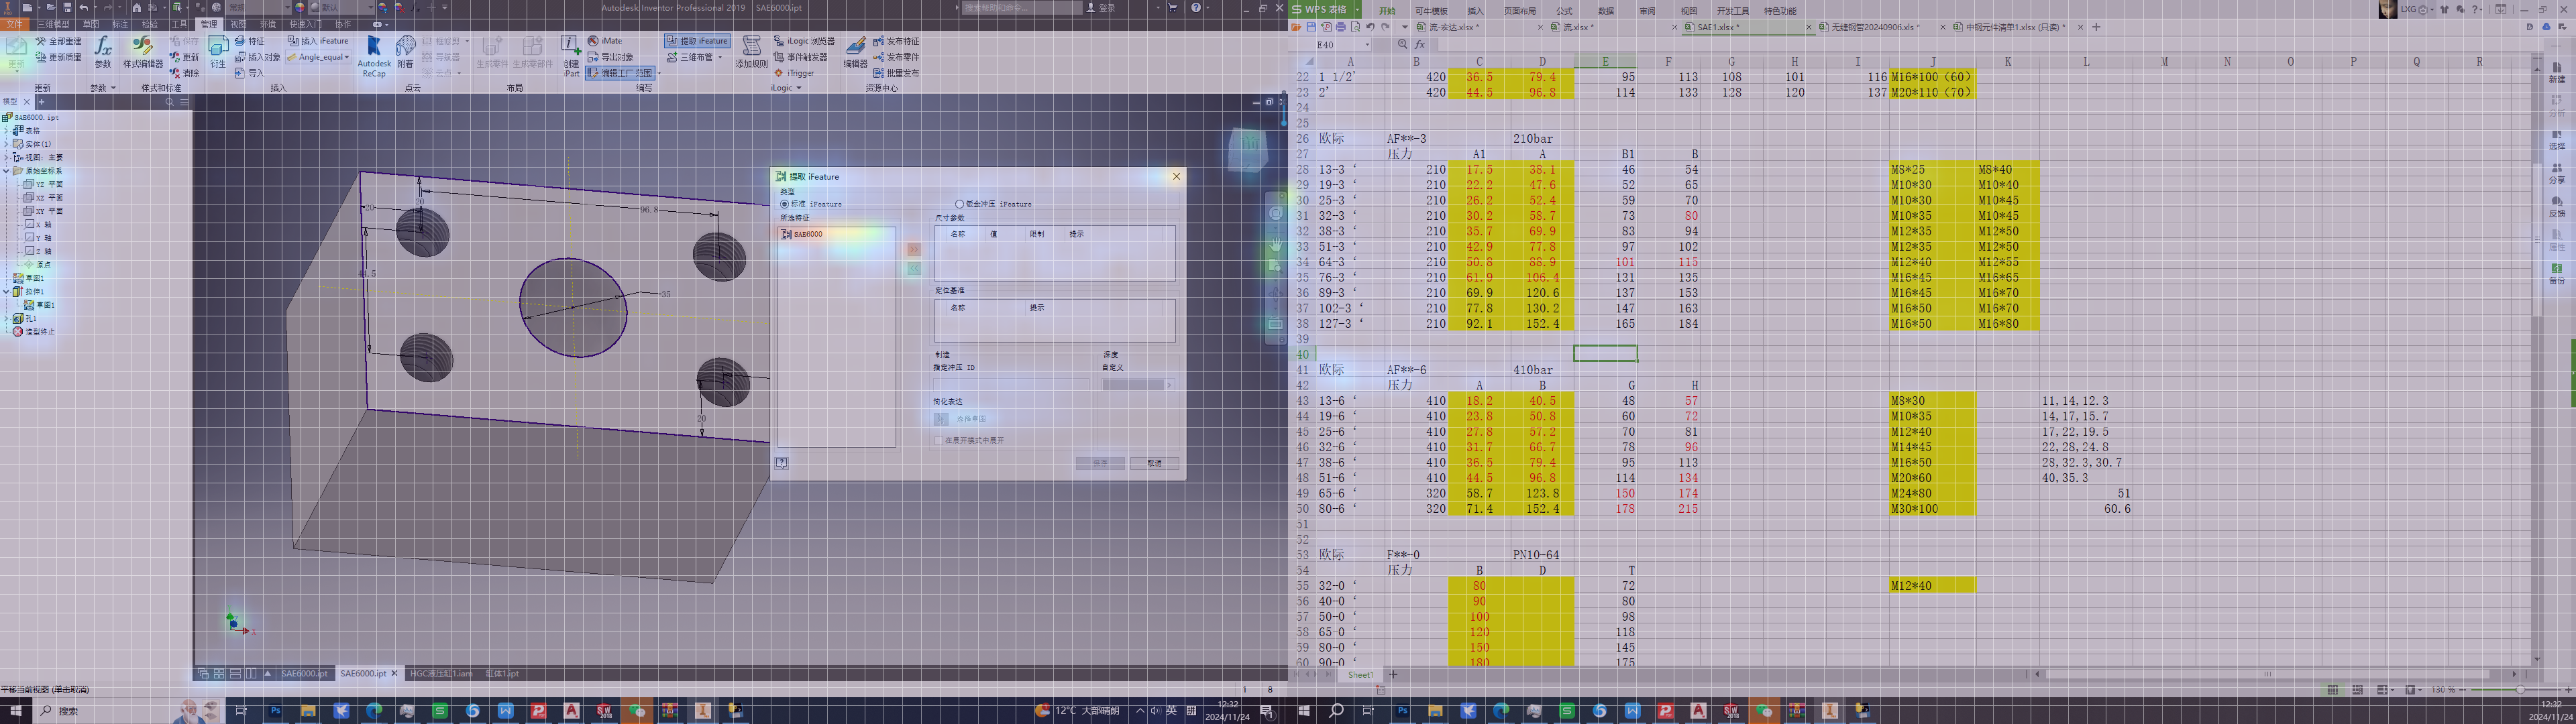
\includegraphics[width=\linewidth]{fig/vis_pro/select.png}
    \caption{Select the only feature.}
\end{subfigure}

\caption{Visualization examples of \method{}'s grounding results on ScreenSpot-Pro.}
\label{fig:example_pro2}
\end{figure}